\label{chap:theory}

This chapter will introduce previous work and background theory needed to develop our approach.
We will first describe the information overload problem, before delving into
how user modeling and recommender systems are currently used to solve this problem.
This chapter will also introduce the field of personalized search, 
where our adaptive recommenders will be especially applicable.

\section{Information Overload}

Information overload conveys the act of receiving \emph{too much information}. 
The problem is apparent in situations where decisional accuracy turns from improving with more information, 
to being hindered by too much irrelevant data \cite[p13]{Bjorkoy2010d}. 
This is a widespread phenomenon, with as many definitions as there are fields experiencing the problem. 
Examples include \emph{sensory overload}, \emph{cognitive overload} and \emph{information anxiety} \cite[p2]{Eppler2004}.
Two common tasks quickly become difficult when this happens:

\begin{enumerate*}
  \item Consumption of relevant content is hindered by too much irrelevant noise.
  \item Discovering new and interesting content is difficult because of too much information.
\end{enumerate*}

\noindent
Finding contemporary examples is not difficult:

\begin{itemize*}
  \item Missing important news articles that get drowned out by irrelevant content.
  \item Forgetting to reply to an email as new messages keep arriving.
  \item Consuming sub-par entertainment because the most relevant is never discovered.
  \item Reformulating search queries because the results include irrelevant items.
  \item Browse through much information to find what one is actually looking for.
\end{itemize*}

Information overload is often likened to a \emph{paradox of choice}, as there may be no problem acquiring the relevant information, 
but rather identifying this information once acquired. As put by \cite[p6]{Edmunds2000}: 
"The paradox --- a surfeit of information and a paucity of useful information."
While normal cases of such overload typically result in feelings of being overwhelmed and out of control, 
\citet[p5]{Bawden2008} points to studies linking extreme cases to various psychological conditions 
related to stressful situations, lost attention span, increased distraction and general impatience.

\cite{Kirsh2000} argues that "the psychological effort of making hard decisions about \emph{pushed} information is the first cause of cognitive overload." 
According to \citeauthor{Kirsh2000}, there will never be a fully satisfiable solution to the problem of overabundant information, 
but that optimal environments can be designed,
in order to increase productivity and reduce the level of stress.
This is achieved through careful consideration of each user's needs. 
In other words, to solve the problems of information overload, 
applications must be able to individually adapt themselves to each user. 

An insightful perspective on information overload comes from the study of \emph{attention economy}. 
In this context human attention is seen a scarce commodity, offset by how much irrelevant noise is present at any given time. 
\citet[p1]{Davenport2001} defines attention as "[...] focused mental engagement on a particular item of information. 
Items come into our awareness, we attend to a particular item, and then we decide whether to act". 
To evade information overload means maximising the available attention, allowing more focus on the most important items in each situation.

\begin{wrapfigure}{rt}{0.5\textwidth}
  \vspace{-20pt}
  \begin{center}
    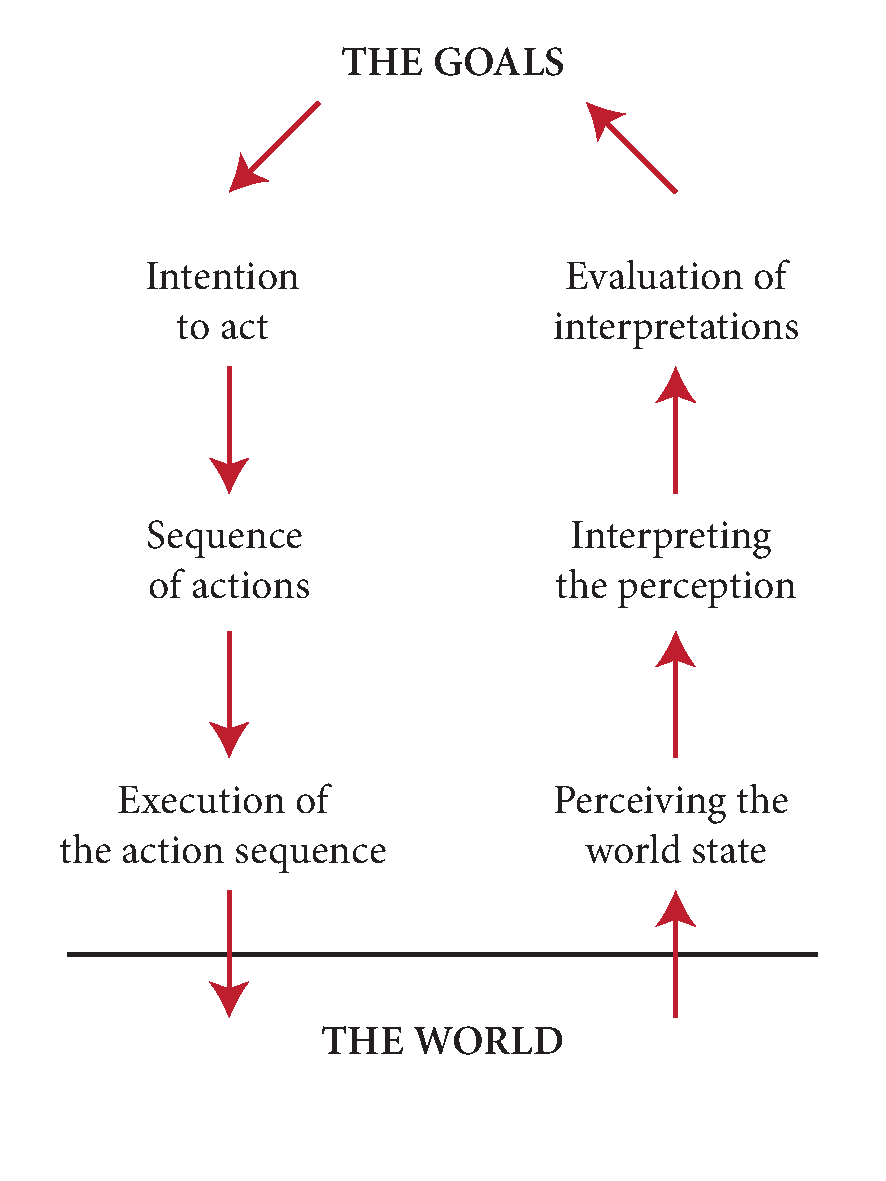
\includegraphics[width=0.5\textwidth]{../graphics/seven-stages.pdf}
    \vspace{-20pt}
    \caption[The Seven Stages of Action]{Stages of Action}
  \end{center}
  \label{fig:seven-stages}
  \vspace{-20pt}
\end{wrapfigure}

Conceptual models used in interaction design can also help us see when and where information overload interferes with a user's experience. 
\cite{Norman1988} advocates a model called \emph{the seven stages of action}, 
that describes how each user goes through several states while using a system
(see Figure \ref{fig:seven-stages}, adapted from \citeauthor{Norman1988}). 
First, the user forms a goal and an intention to act. The user then performs a sequence of actions on the world (the interface)
 meant to align the perceived world and the goals. After performing a set of actions, the new world state is evaluated and perceived. 
At last, the user evaluates the perception and interpretation of the world in accordance with the original goal.

As apparent from this model, information overload can interfere both before and after any action is taken. 
For example, if the application presents too much content, or presents content in a confusing manner, 
it can be difficult for the user to identify which actions that would help achieve the current goal. 
Likewise, after actions are taken, the new world state can suffer the same shortcomings of overwhelming scope or lack of presentations, 
leading to information overload. 
This precludes the user from properly evaluating the resulting application state. 

In short, an application interface can fail both before and after a user tries to interact with it.
Information overload happens throughout the interaction process.


\subsection{Online Overload}

The Web is a common source of information overload, 
and a good example of how and why the problem occurs.
Online information overload is especially pervasive when considering \emph{content aggregating websites}:
Web sites that combine information from multiple other sites and sources. 
Online information retrieval systems (search engines) are in category, as are
online newspapers, feed readers and portal sites.

The wealth and scope of data on the Web are natural culprits of online overload, 
as well as the varying qualities of websites publishing the information. 
However, the problem is also a result of the fundamental observed structure of the Web.
Graph theory presents applicable models that characterize how people navigate between websites, 
and show how content aggregators form important hubs in the network. 
These models give a theoretical foundation for why information overload occurs on the Web.

In the Web graph, nodes correspond to websites and
directed edges between nodes are links from one page to another. The \emph{degree} of a node is defined as its number of edges.
This graph has the properties of a \emph{small-world network} (\citep{Newman2000}, \citep[p2]{Huang2005}), 
a type of random graph, where most nodes are not neighbors, but most nodes are reachable through a small number of edges (See Figure \ref{fig:swn}). 
This is because of important random shortcuts differentiating the graph from a regular lattice. 
The graph is not  random, but neither is it completely regular.
As described by \citet[p37]{Barabasi2003}, the average number of outbound links from a web page is around 7.
From the first page, we can reach 7 other pages. From the second, 49 documents can be reached. 
After 19 links have been traversed, about $10^{16}$ pages can be reached (which is more than the actual number of existing web pages, since loops will form in the graph).
%\footnote{The concept of small-world networks came from the observation that there is often a surprisingly short minimum distance between nodes in an average graph. This is called the small world phenomenon, and is often mentioned alongside the concept of "six degrees of separation", popularized in a play by John Guare. This concept states that no person is on average more than six social links removed from any other person on earth.}

\begin{figure}[t]
  \includegraphics[width=\textwidth]{../graphics/graphs}
  \caption[Examples of Complex Networks]{
    Complex Networks,
    from the left: A \emph{random} network, a \emph{small-world} network and a \emph{scale-free} network 
    (which is a type of  small-world network). Figure adapted from \citep[p2]{Huang2005}.} 
  \label{fig:swn}
\end{figure}


The high degree of the Web graph would suggest that finding an optimal path to your desired page is quite difficult. 
Yet, while it is true that finding the \emph{optimal path} is hard, finding \emph{a good path} is not that big a challenge. 
When people browse the Web, links are not followed blindly --- 
we use numerous heuristics to evaluate each link, often resulting in quite a good path to where we want to go. 
So why is the Web still quite challenging to navigate?

As discovered by \cite{Albert1999}, the Web also exhibits properties of a \emph{Scale-Free Network} (\smallcaps{SFN}). 
They found that in some natural observed networks, there exists a small number of nodes with an extremely high degree. 
This is also true on the Web --- some websites have a huge number of outbound links. 
For comparison, while a random network is similar to a national highway system, with a regular number of links between major cities, scale-free networks are more like an air traffic system, with central hubs connecting many less active airports \citep[p71]{Barabasi2003}.

These highly connected nodes, called \emph{hubs}, are not found in small-world networks or random graphs. As demonstrated by the presence of hubs, the degree distribution of a scale-free network follows a power law, 
$P(k) \sim k^{-\gamma}$, 
where $P(k)$ is the probability of a node having k connections and $\gamma$ is a constant dependent on the type of network, typically in the range $2 < \gamma < 3$. 
Since the Web has directed edges,
we have two power laws:
$P_{in}(k) \sim k^{-\gamma_{in}}$ and 
$P_{out}(k) \sim k^{-\gamma_{out}}$.

\cite{Albert1999} describes a number of studies placing the $\gamma$ values for the Web in the $[2,3]$ range, 
with $\gamma_{out}$ being slightly higher than $\gamma_{in}$. 
Both these probabilities exhibit power tails (or long tails). 
In other words, a few important nodes have a huge number of inbound and outbound links --- the hubs. 
\citet[p86]{Barabasi2003} proposed that hubs emerge in a scale-free networks because of two factors:
(1) Growth: Nodes are added to the network one by one, for example when new websites are added to the Internet.
(2) Preferential attachment: When new nodes are created, they connect to existing nodes. The probability that the new node will connect to an existing node is proportional to the number of links the existing node has. In other words, older, more established and central nodes are preferred neighbors.
This is called the Barab\'{a}si-Albert model \citep{Albert1999}, 
and the probability for a new node connecting to an existing node is given by $\prod k_i$, 
where $k_i$ is the number of links pointing to node $i$, in the following equation: 

\begin{eqsp}
  \prod_{i} k_i  = \frac{k_i}{\sum_{j}^N k_j}.
\end{eqsp} 
%
Search engines, social link aggregators, news portals, et cetera are all hubs of the Internet, emerging from the preferential 
link attachment of newly created nodes, that make navigating the Web less easy as it might appear.
What does seem clear is that these content aggregating hubs are prime candidates for overwhelming their users with information. 
The fundamental observed structure of the Web creates the need for information brokers that link the net together, 
and the need for techniques to display a lot of data --- adapted to each user and each item.
In other words, we need user modeling, that can predict how relevant each item will be for each user.
 


\section{User Modeling}
\label{sec:modeling}

The term \emph{user modeling} (\smallcaps{UM}) lacks a strict definition. 
Broadly speaking, when an application is adapted in some way based on what the system knows about its users, we have user modeling. 
From predictive modeling methods in machine learning, 
to how interface design is influenced by personalization, the field covers a lot of ground. 

It is important to differentiate between adapting the interface of an application and the content of an application. 
Many user modeling methods strive to personalize the interface itself, e.g. menus, buttons and control elements 
(e.g. \cite{Jameson2009, Fischer2001}). 
Adapting the content, on the other hand, means changing how and what content is displayed.
For instance, interface adaption might mean changing the order of items in a menu, while content 
adaption might mean changing the order and emphasis of results in a web search interface
(e.g. \cite{Xu2008, Qiu2006, Rhodes2000}).

In this thesis, we are interested in adapting the \emph{content} of an application.
We believe the information overload problem often stems from a mismatch between presented content and desired content. 
Examples of adaptive content include:

\begin{itemize*}
  \item Suggesting interesting items based on previous activity.
  \item Reorganizing or filtering content based on predicted user relevance.
  \item Translating content based on a user's geographical location.
  \item Changing the presentation of content to match personal preferences or abilities.
  \item Personalizing search results based on previous queries and clicks.
\end{itemize*}

The fields of Artificial Intelligence (AI) and Human-Computer Interaction (HCI) share a common goal solving information overload through user modeling. 
However, as described by \cite[p.6]{Lieberman2009}, they have different approaches and their efforts are seldom combined. 
While AI researchers often view contributions from HCI as trivial cosmetics, the HCI camp
tends to view AI as unreliable and unpredictable --- surefire aspects of poor interaction design.

In AI, user modeling refers to algorithms and methods that infer knowledge about a user based on past interaction 
(e.g. \cite{Pazzani2007, Smyth2007, Alshamri2008, Resnick1994}).
By examining previous actions, predictions can be made of how the user will react to future information. This new knowledge is then embedded in a model of the user, which can predict future actions and reactions. 
For instance, an individual user model may predict how interesting an unseen article will be to a user, based on previous feedback on similar articles or the feedback of similar users.

HCI aims to meet user demands for interaction. 
User modeling plays a crucial role in this task. 
Unlike the formal user modeling methods of AI, user models in HCI are often cognitive approximations, manually developed by researchers to describe different types of users 
(e.g. \cite{Fischer2001, Jameson2009, Cato2001}).
These models are then utilized by interaction designers to properly design the computer interface based on a models predictions of its user's preferences.
\cite{Totterdell1990} describes user modeling in interaction design as a collection of deferred parameters: 

\begin{blockquote}
  ``The designer defers some of the design parameters such that they can be selected or 
  fixed by features of the environment at the time of interaction [...] 
  Conventional systems are special cases of adaptive systems in which the parameters have been pre-set.'' 
\end{blockquote}

This thesis is concerned with the AI approach to user modeling, and in particular, the use of \emph{recommender systems} (RSs).

\subsection{Interface Autonomy}

\begin{figure}[t]
  \includegraphics[width=\textwidth]{../graphics/autonomy.pdf}
  \caption[Levels of Interface Autonomy]{
    Levels of Interface Autonomy:
    Interfaces range from those only customizable by the user, 
    to intelligent systems takes the initiative on their own accord.
  }
  \label{fig:autonomy}
\end{figure}

Using AI to adapt an interface raises important questions with regard to usability, privacy and usefulness.
These questions are rooted in the autonomy expressed by each interface.
An autonomous interface is one that takes initiatives on its own, regardless of whether the user has asked for it \cite[p.2]{Lieberman}. 
Naturally, any application that automatically personalizes its content will be autonomous to some degree.

Adaptive interfaces can be classified into increasing order of autonomy (see Figure \ref{fig:autonomy}). 
At the order of least autonomous systems, we have \emph{customizable interfaces}. 
These are interfaces that the user may customize themselves, but that do not take the initiative or change anything without explicit user action. 
For example, an interface might have a settings panel where users can change the order of items in a menu.

At the next level of autonomy, we have \emph{adaptive interfaces} that suggest to the user possible changes or actions that might be beneficial. For example, an email application could suggest which folder an email should be moved to.
At the most autonomous level, \emph{intelligent interfaces} implicitly and automatically customize the interface or content based on passive observation of the user. 
This could for instance entail automatic filing of emails based on content classification and data mining of previous user actions with similar messages.

An application that personalizes content automatically will fall somewhere in the two last categories and present either an adaptive or intelligent interface, 
depending on the extent and transparency of its autonomy.

In this thesis, we are only interested in fully autonomous, intelligent interfaces.
We will create a system that implicitly, and without any effort from each user,
can adapt the content of an application based on previous behavior.
Other examples of such implicit user modeling include \cite{Qiu2006}, \cite{Shen2005} and \cite{Carmel2009}.

As our goal is to adaptively combine different RSs based on each user and item,
we shall now describe what makes a recommender system, and introduce some of the many algorithms they employ.

\section{Recommender Systems}

The name might seem constraining, but recommender systems are incredibly powerful methods in user modeling.
Whenever we wish to predict the relevance of an item to a user, recommender systems are the tools to use.
Such systems are commonly used on the web to provide a host of predictive functionality, including:

\begin{itemize*}
  \item Recommending products like books or movies based on past purchases.
  \item Suggesting new social connections based on an existing social graph.
  \item Recommending items based the activity of similar or like-minded users.
  \item Ordering news articles by predicted individual relevance.
\end{itemize*}

Common to these examples are a set of users, a set of items, and a sparse set of explicit ratings or preferences.
A recommender system is best described as a graph, even though the underlying algorithms might not use this as the representation.
\cite{Mirza2003} explains how any RS can be expressed as a graph traversal algorithm.
Items and users are nodes, while ratings, social connections et cetera are edges between the nodes.
An RS performs predictive reasoning on this graph by estimating the strenghts of hypothetical connections between nodes that are not explicitly connected.

For example, if a user has rated some of the movies in a movie recommendation system, 
we use these ratings to predict how well the user will like unseen movies,
based on a movies ratings from users similar to the one in question.
In social networks, recommender systems can be used to infer new social relations 
based on existing connections. The principle is the same: By evaluating current explicit
connections, and the connections of similar users, new connections can be predicted.
Recommender systems are then powerful methods for user modeling, personalization and fighting information overload,
because of their ability to infer how relevant and item (or another user) will be to the current user.

Formally, a recommender system is a quintuple, $\mathrm{RS} = (I, U, R, F, M)$,
where $I$ is the set of items (e.g. products, articles or movies) and $U$ is the set of users.
$R$ is the set of known ratings, i.e. explicit preferences given by users for certain items.
$F$ is a framework for representing the items, users and ratings, and 
$M$ is the actual modeling method used to infer unknown ratings 
for predicting a user's preference for an unrated item. 

In \cite{Adomavicius2005}, $M$ is seen as a utility function
$f: U \times I \rightarrow S$. Here, $f$ is a function that maps the set
of users and items into a fully ordered set of items $S$, ranked by their
utility (i.e. rating) to each user. In other words, $S$ is the complete version of $R$,
where each user has either an explicit or predicted preference for each item in $I$.
In this notation, to predict the best unrated item for each user, we simply find the item with the highest expected utility:

\begin{eqnarray*}
  \forall u \in U,\text{ } i'_u = \arg\max_{i \in I} f(u,i)
\end{eqnarray*}

The utility function $u$ depends on the modeling method being used, the active user and the item in question. 
The \emph{reason} for using a recommender system is that the utility $u$ is not defined for the entire $U \times I$ space, 
i.e. the system does not explicitly know the utility of each item for each user. 
The point of a recommender system is then to extrapolate $u$ to cover the entire user-item space. 
In other words, to be able to rank items according to user preferences, 
the system must be able to predict each user's reaction to items they have not yet explicitly rated themselves. 
This is where predictive user models come in handy.

Another popular way of describing, and implementing an RS is using a simple matrix. 
Here, one dimension represents users, the other dimension represents items,
and each cell corresponds to an explicit rating. This matrix then becomes the framework $F$ in our 
RS quintuple:

\begin{eqnarray*}
 R_{m,n} =
 \begin{pmatrix}
  r_{1,1} & r_{1,2} & \cdots & r_{1,n} \\
  r_{2,1} & r_{2,2} & \cdots & r_{2,n} \\
  \vdots  & \vdots  & \ddots & \vdots  \\
  r_{m,1} & r_{m,2} & \cdots & r_{m,n}
 \end{pmatrix}
\end{eqnarray*}

Critically, these matrices are usually extremely sparse (i.e. most of the cells are empty). 
Consider that while there may be a large number of users and items, each individual user
only rates or connects to a few number of items. 
For example, in the seminal Netflix Challenge movie recommender dataset, almost 99\% of the potential
user/item pairs have no rating \citep[p1]{Bell2007d}. In other words, the recommender system must be able
to produce results from a matrix where only 1\% of the cells have meaningful values.

Naturally, this is the defining characteristic of 
many recommender systems: the ability to extract meaningful patterns from sparse data, 
through dimensionality reduction, neighborhood estimation and similar methods.

Recommender systems face many challenges other than the sparsity problem.
A directly related problem is the need for large datasets. Since the data is often sparse,
the systems will most often perform well if used on large numbers of items and users.
As in many machine learning methods, concept drift, where the characteristics of a user or item
changes over time, is also eternally present.
Finally, the performance of RSs is often closely tied to their computational complexity. 
Real world usage of the most precise methods is often hindered by the computational power
needed to actually put them into production.




\subsection{Estimation of Ratings}

The most interesting and important part of any RS is how it predicts unknown ratings.
(Note that altough we use "ratings", "utility", "preference", "relevance" and "connection strength" depending on the context, they all basically mean the same.)
Because of this, each method is best categorized based on a few dimensions of its predictive capabilities (see Table \ref{table:taxonomy}).
In our taxonomy, these dimensions are: Predictions, method, granularity, temporality and agents.

\begin{table}[b]
  \begin{tabular*}{\textwidth}{ p{3cm} l @{\extracolsep{\fill}} }
    \toprule
    \emph{Variable} & \emph{Values} \\
    \midrule
    Predictions & Content-based | Collaborative | Hybrid\\
    Method & Heuristic | Model-based\\
    Granularity & Canonical | Typical | Individual\\
    Temporality & Short-term | Long-term\\
    Agents & Implicit | Explicit\\
    \bottomrule
  \end{tabular*}
  \caption[Recommender Systems Taxonomy]{A taxonomy of recommender systems. From \cite{Bjorkoy2010d}.}
  \label{table:taxonomy}
\end{table}

The \emph{predictions} variable represents what data the RS uses to perform predictions. 
Content-based methods use only the items, inter-item relations, and 
an individual user's past history as predictive of future actions \citep{Pazzani2007}.
By only considering the individual user in adapting an application, highly personal models can be created. 
However, such methods often require a lot of interaction before reliable models can be created \citep{Adomavicius2005}.
The problem of having to do complex inference from little data, as is often is in content-based predictions, is often called the \emph{sparsity problem} or the \emph{cold start} problem. This is closely related to the problem of \emph{overfitting} data, where the algorithms creates models that match the training data, but not the actual underlying relationships. A lot of research looks at ways to overcome sparse data, i.e. achieving "warmer" cold start. 
When using content-based predictions, the utility function $f(u,i)$ of user $u$ and item $i$ is extrapolated from $f(u,i_u)$, 
where $i$ is an item similar to $i_u$ and $f(u,i_u)$ is known.

Collaborative or social recommendations build predictive models for users based on the actions of similar users 
\citep{Schafer2007}.
The observation is that similar users should have similar usage and action patterns. 
By using data from more than one user, expansive models may be built. 
These methods are especially useful when considering new users of a service. 
A central problem with collaborative methods is that the resulting model is not as individually tailored as one created through content-based learning. 
Collaborative models must be careful not to represent the \emph{average} user, but a single individual.
When using collaborative learning, 
the utility $f(u,i)$ of item $i$ for user $u$ is extrapolated from $f(u_j,i)$ where $u_j$ is a user similar to $u$. 

Because of \emph{the new user problem} of content-based learning and the \emph{average user problem} of collaborative learning, 
many systems use a hybrid approach \citep{Burke2007}.
By combining content-based and collaborative learning, 
systems that properly handle predictions for new users and avoid too much generalization in the models can be achieved. 

The \emph{method} variable, is another way to classify recommenders. Orthogonal to what data the method uses, this variable
concerns \emph{how} the data is used to produce recommendations.
First we have the \emph{model-based} approach, where the recommender system builds predictive models based on the known data. 
Unseen items can then be fed into this model to compute its estimated utility score. 
For example, creating a Bayesian networks from past interaction is a model-based approach.
The other category is the \emph{heuristic} or \emph{memory-based} approach. 
These methods use the raw data of items, users and ratings to directly estimate unknown utility values. 
For example, recommending items similar to the ones already rated by computing the cosine similarity of their feature vectors is a heuristic approach.


The \emph{granularity} variable tells whether this approach creates models for the canonical user, stereotypical users or individual users. 
\cite{Rich1979} presented one of the first user modeling systems based on stereotypes, used to predict which books in a library each user would most enjoy.
Here, a dialogue between the system and the user was performed to place the user into a set of sterotypes. 
Each stereotype has a set of \emph{facets} which is then used to match books and users.

\emph{Temporality} refers to how volatile the gathered knowledge will be.
While most RSs produce long term, relatively stable knowledge based on lasting user preference and taste, 
some systems use fluctuating parameters such as the time of day, exact location and the current context to produce recommendations.
For example, \cite{Horvitz} used clues from a user's calendar, camera and other sensors to determine the attentional state
of the user before delivering personalized and contextual notifications.

The \emph{agents} variable signifies whether the knowledge gathering and presentation is implicit and opaque, 
or explicit and requires dedicated user interaction. Explicit feedback through ratings is 
common in movie, product or music rating services (e.g. \cite{Bell2007, Basu1998, Hotho}). However, for other services such as personalized search,
implicit mining of query logs and user interaction is often used to build user models (e.g. \cite{Shen2005, Agichtein2006, Speretta2000, Teevan2005})


\subsection{Approaches}

Because our solution will combine different recommender systems, we need a short introduction to some of the approaches we will combine.

TODO

\subsection{Examples of Recommender Systems}
\label{subsec:recommender:examples}

As our solution will combine different recommender systems, we need a short introduction to some of the approaches we will use.
Let us take a closer look at (1) \emph{baseline ratings}, (2) \emph{neighborhood estimation}, (3) \emph{dimensionality reduction}, 
and (4) \emph{network traversal}. This is by no means an exhaustive list, but rather
a quick rundown of common approaches in recommender systems, that we will use in the Chapter \ref{chap:methods}.
See \cite{Adomavicius2005}, \cite{Pazzani2007}, \cite{Schafer2007} or \cite{Bjorkoy2010d} for a more comprehensive exploration of different types of recommenders.
\cite{Segaran2007} gives a good introduction to how RSs are used in practice.

(1) \emph{Baseline ratings} are the simplest family of recommender systems.
These methods compute predictions through varying types of averages of known data.
The data is content-based, and used to compute heuristic predictions.
While simple in nature, these methods are often helpful starting points for more complex systems, or as 
benchmarks for exploring new approaches. 
For example, \citet[p2]{Koren2008} computes the baselines for items and users, and
use more involved methods to move this starting point in some direction. 
The baseline (predicted relevance) for a user/item pair is given by

\begin{eqsp}
  b_{ui} = \mu + b_u + b_i
\end{eqsp}
%
where $\mu$ is the average rating across all items and users, 
$b_u$ is the user baseline and 
$b_i$ is the item baseline.
The user and item baselines correspond to how the user's and item's ratings deviate from the norm.
This makes sense as some items may be consistently rated higher than the average, some users may be 
highly critical in their assessments, and so on. \citeauthor{Koren2008} computes these baselines by solving the
least squares problem

\begin{eqsp}
  \min_{b*} = \sum_{(u,i) \in R} (r_{ui} - \mu - b_u - b_i)^2 + \lambda ( \sum_{u} b_u^2 + \sum_{i} b_i^2 )
\end{eqsp}
%
which finds baselines that fit the given ratings while trying to reduce overfitting
by punishing greater values, as weighted by the $\lambda$ parameter. 
By using baselines instead of simple averages, more complex predictors gain a better starting point,
or in other words, a better average rating.

Another approach based on simple averages is the  \emph{Slope One} family of recommender algorithms. 
As introduced by \cite{Lemire2005}, these algorithms predict unknown ratings based on the average difference in ratings between two items. 
For example, if item $i$ is on average rated $\delta$ points above item $j$, and user $u$ has rated item $j$,
that is, we predict $\hat{r}_{u,i}$ (the estimated rating) to be $r_{u,j} + \delta$, for all the user's ratings that match this pattern,

\begin{eqsp}
  \hat{r}_{u,i} = \frac{\sum_{j \in R_u} \mathrm{ratings}(j) \times (r_{u,j} + \mathrm{\delta}(i,j))}{\sum_{j \in R_u} \mathrm{ratings}(j) }.
\end{eqsp}

Here, $\hat{r}_{ui}$ is the estimated rating, $R_u$ is the items rated by user $u$, $\mathrm{ratings}(i)$ is the number of ratings for item $i$,
and $\mathrm{\delta}(i,j)$ is the average difference in ratings for items $i$ and $j$.
While simplistic, Slope One is computationally effective and produces results comparable to more complex methods \cite[p5]{Lemire2005}.

(2) \emph{Neighborhood estimation} is at the core of many recommendation systems. 
This is the basic principle behind most collaborative filtering algorithms. 
Unknown ratings are estimated by averaging the ratings of similar items or users, weighted by their similarity.
Neighborhood-based approaches often work in two steps. First, a neighborhood if similar elements is computed.
second, the similarities and connections within this neighborhood is used to produce a prediction.

A common method for computing user similarity is the \emph{Pearson Correlation Coefficient} (PCC) \cite[p11]{Segaran2007}.
While simple, the PCC compares favorably to more complex approaches, and is often used as a benchmark 
for testing new ideas (e.g. in \citet{Lemire2005, Ujjin, Konstas}).

The PCC is a statistical measure of the correlation between two variables. In our domain, the variables
are two users, and their measurements are the ratings of co-rated items. 
The coefficient produces a value in the range $[-1,1]$ where $1$ signifies perfect correlation (equal ratings),
$0$ for no correlation and $-1$ for a negative correlation.
The negative correlation can signify two users that have diametrically opposing tastes.
We compute PCC by dividing the covariances of the user ratings with their standard deviations:

\begin{eqsp}
  \mathrm{pcc}(u,v) = \frac{cov(R_u, R_v)}{\sigma_{R_u} \sigma_{R_v}}.
\end{eqsp}

When expanding the terms for covariance and standard deviations, 
and using a limited neighborhood size $n$, we get

\begin{eqsp}
  \mathrm{pcc}_{n}(u,v) = 
    \frac{
      \sum_{i \in K}^{n} (R_{ui} - \bar{R_u}) (R_{vi} - \bar{R_v}) }{ 
        \sqrt{ \sum_{i \in K}^{n} (R_{ui} - \bar{R_u})^2 } 
        \sqrt{ \sum_{i \in K}^{n} (R_{vi} - \bar{R_v})^2 }}.
\end{eqsp}

The limited neighborhood size becomes the statistical sampling size, and is a useful
way of placing an upper bound on the complexity of computing a neighborhood.
$n$ does not have to be a stochastic sampling --- it can also be limited by the number of ratings 
the two compared users have in common, the number of ratings each user have, or something similar,
as denoted by $K$ in the formula.

After a neighborhood is determined, it is time to predict the unknown rating.
For Collaborative filtering approaches, we are interested in the similarity of users,
which means averaging the user neighborhood ratings weighted by similarity \cite[p16]{Segaran2007}:

\begin{eqsp}
  \bar{r}_{ui} = \frac{ \sum_{v \in K(u,i)} \mathrm{sim}(u,v) \times R_{vi} }{ \sum_{v \in K(u,i)} \mathrm{sim}(u,v) },
\end{eqsp}
%
where $\mathrm{sim}(u,v)$ is the similarity between two users, $K(u,i)$ is the set of users in the neighborhood of $u$ that have rated item $i$.
This is one of the simplest ways of computing a neighborhood-based prediction.
Most systems use more complex estimations. For instance, \cite{Koren2008} 
uses the baseline ratings discussed above instead of plain user and item ratings, to
remove what they call global effects where some users are generous or strict in their 
explicit preferences, and some items are consistently rated differently than the average.

\emph{Content-based} recommenders compute neighborhoods if items instead of users.
The simplest approach is to find items highly rated by the current user, compute the neighborhood 
by finding items similar to these, and produce ratings by weighting the initial rating
with the similarity of the neighboring items.

The PCC is but one of many methods used to compute neighborhoods. 
Other simple measures include the \emph{euclidean distance} \cite[p10]{Segaran2007},
Spearman's or Kendall Tau rank correlation coefficients \cite[p30]{Herlocker2004} --- 
variations on the PCC.
Of course, user similarity does not have to rely on ratings. 
If the system has access to detailed user profiles, these can be used
to estimate the similarity of users.
Similarity metrics from the field of \emph{information retrieval} (IR),
such as the \emph{cosine correlation} of rating vectors,
or content-based similarity metrics are applicable,
as we shall see in Section \ref{sec:search}.

\cite{Bell2007a} shows a more sophisticated neighborhood estimation which computes global interpolation weights,
that can be computed simultaneously for all nearest neighbors.
Combinations of different types of neighborhoods are also possible. 
\cite{Ujjin} use a simple euclidean metric to gather a larger neighborhood, which is then refined using a \emph{genetic algorithm}.
Another common way of computing neighborhoods is by reducing the dimensions of the ratings matrix, as we will now describe.

(3) \emph{Dimensionality reduction} is an oft-used technique when creating recommender systems.
The ratings matrix is factored into a set of lower dimension matrices, that can be used to approximate the original matrix.
By reducing the noise in the ratings matrix, and keeping those ratings that contribute to global patterns,
we can identify groups of users, items or combinations that have something in common.
This can then be used to find neighborhoods, compute similarities and estimate unknown ratings.

\emph{Singular Value Decomposition} (SVD) is a common method for such matrix factorization (e.g. \citet[p5]{Billsus}, \citet{Sun2005}, \citet{Bell2007}).  
This is the same underlying technique used by \emph{latent semantic indexing} in information retrieval \cite[p44]{Baeza-Yates1999}.
Formally, SVD is the factorization $R = U \Sigma V^{T}$. 
$R$ is an $m \times n$ matrix, in our case the ratings matrix, with $m$ users and $n$ items. 
$U$ is an $m \times m$ factor, $V^{T}$ (the transpose of $V$) is an $n \times n$ factor.
$\Sigma$ is a $m \times n$ diagonal matrix. 
$\Sigma$ is a diagonal matrix, made up of what is called the \emph{singular values} of the original matrix.

The dimensionality reduction can be performed by truncating the factor matrices each to a number of rows or columns, 
where the number is a parameter depending on the current domain and data, called the $rank$ ($r$).
The truncated matrix is $R_r = U_r \Sigma_r V_r^{*}$, where $U_r$ are the first $r$ columns of $U$,
$V_r^{T}$ are the first $r$ rows of $V^{T}$ and $\Sigma_r$ is the top-left $r \times r$ sub-matrix of $\Sigma$.
There are many more complex ways of compressing the matrix than pure truncation, but this is a common way of reducing the factors.
By truncating the factors, we in essence create a higher-level approximation of the original matrix that can identify latent features in the data.
With the factors reduced to $r$ dimensions, the resulting matrices are compressed:

\begin{eqsp}
  \begin{bmatrix}
    { } & { } & { }     & { } & { }\\
    { } & { } & { }     & { } & { }\\
    { } & { } & R_{m,n} & { } & { }\\
    { } & { } & { }     & { } & { }\\
    { } & { } & { }     & { } & { }
  \end{bmatrix} 
  \quad 
  \Rightarrow
  \quad
  \begin{bmatrix}
    { }\\
    { }\\
    U_{m,r}\\
    { }\\
    { }
  \end{bmatrix}
  %\quad
  \begin{bmatrix}
    \Sigma_{r,r}
  \end{bmatrix}
  %\quad
  \begin{bmatrix}
    { } & { } & V_{r,n}^{*} & { } & { }\\
  \end{bmatrix} 
\end{eqsp}
%
Two important transformations happen in this dimensionality reduction. 
First, ratings that do not contribute to any greater pattern are removed as noise.
Second, ratings that in some way correlate to each other are enhanced, giving more weight to the actual predictive parts of the data.
This means that the reduced factors can for instance identify features that correspond to correlations between items or users.
These features are comparable to the mapping of terms to concepts in LSI.

\begin{figure}[t]
  \includegraphics[width=\textwidth]{../graphics/compression}
  \caption[SVD Image Compression]{
    SVD Image Compression:
    A variation of using SVD to compress an image, from \cite{Ranade2007}.
    The original image is on the left, and successive images use an increasing number of factors (2, 8 and 30) when performing compression.
    Figure adapted from \citet[p4]{Ranade2007}.
  }
  \label{fig:svd-image}
\end{figure}

Because SVD can find the most descriptive parts of a matrix, this technique is often used for image compression.
The image we wish to compress is treated as an $N \times M$ matrix, which is run through an SVD factorization.
The factors are truncated, and the result expanded to a matrix that is much simpler to represent
than our original image matrix. As seen in Figure \ref{fig:svd-image}, how close the compressed image resembles the original image
depends on the chosen $rank$, i.e. how many rows and columns we keep during truncation.
A higher rank means less dimensionality reduction and less compression of the image.

The key question for any SVD algorithm is how it performs the factorization,
and which rank the original matrix is reduced to.
Two common factorization methods are the EM and the ALSWR algorithms.
An EM factorizer uses the Expectation-Maximization algorithm to find the factors.
An ALSWR factorizer performs the same factorization with a least-squares approach \citep{Zhou2008}.
The number of features refers to the truncation of the factors in order to reduce the concept-space.
These features then correspond to the number of latent taste categories we wish to identify.
Naturally, different numbers of features will yield different recommenders.
The SVD factorization algorithms are iterative methods, where each iteration
yields more accurate results.

In recommender systems, SVD is used to compress the ratings space into what is sometimes called a \emph{taste space},
where users are mapped to higher-level \emph{taste} categories
(e.g. \citet[p5]{Ahn2004}, \citet[p4]{Brand2003} or \citet[p2]{Liu2006}).
In a taste space,
the collections of individual ratings are reduced to groups of users, items and combinations that have patterns in common.
This reduction makes it easy to find similar users that share some global characteristic.
We can also find similarities between items, clusters of items and user and so on, all based on latent categories
discovered by the automatic identification of patterns in the data.
SVD is then an ingenious way of dealing with the commonly sparse ratings data, by identifying latent correlations and patterns in the data,
which is exactly what we need to predict unknown ratings or connections.

(4) \emph{Network traversal recommenders} refers to estimating predictions by traversing a graph of users and items to provide recommendations.
The connections between nodes can be any type of relation that makes sense to the RS. Examples include linking item and user nodes
based on purchases or explicit ratings, linking user nodes from asymmetrical (directed edges) symmetrical (undirected edges) relations,
or linking items based on some similarity metric.
Recommender systems can use common graph-traversal algorithms to infer unknown connections in this graph.

\cite{Huang2002} used network traversal to create a simple system for recommending books to customers.
Here, edges between items and users correspond to ratings, and edges connecting nodes of the same type
are created by connecting elements that have similarity above a certain threshold. Predictions are generated
by traversing the graph a preset number of steps starting at the current user, and multiplying the weights
of paths leading to the target item (see Figure \ref{fig:book-graphs}).

\begin{figure}[t]
  \centering
  \subfloat[]{\label{fig:graph-layers}
    \includegraphics[width=0.5\textwidth]{../graphics/graph-layers}}                
  \subfloat[]{\label{fig:graph-layers-detail}
    \includegraphics[width=0.5\textwidth]{../graphics/graph-layers-detail}}
  \caption[Example of Network Traversal]{Network Traversal Example: (a) A graph with two kinds of nodes,
    e.g. items and users. (b) A graph with books and customers, where recommendations
    can be made by traversing the weighted connections. Connections between nodes of the same type
    represent similarity, while connections between books and customers represent purchases.
    Figures from \cite{Huang2002}.}
  \label{fig:book-graphs}
\end{figure}
%
The complexity of recommender systems based on networks are only limited by the kinds of relations we can produce.
For example, recommending other users in social networks can easily utilize friend or friend-of-a-friend relations
to find others the current user might be interested in connecting to. Indeed, any relevant similarity metric can be used to
connect nodes of the same type, or nodes of different types.

One variation comes from \cite{Walter2008}, who create a network of \emph{transitive trust} to produce recommendations. Here,
the neighborhood of users is determined by traversing through users connected by a level of trust. 
The trust can for example be a function of how many agreeable results the connection to a user has produced.
Uers trust each other's recommendations based on previous experience.

\cite{Konstas} takes yet another approach that measures the similarity between two nodes through their \emph{random walks with restarts} (RWR) technique.
Starting from a node $x$, the RWR algorithm randomly follows a link to a neighboring node. 
In every step, there is a probability $\alpha$ that the algorithm will restart its random walk from the same node, $x$. 
A user-specific column vector $P^{(t)}$ stores the long term probability rates of each node, 
where $P^{(t)}_i$ represents the probability that the random walk at step $t$ is at node $i$. 
$S$ is the column-normalized adjacency-matrix of the graph, i.e. the transition probability table. 
$Q$ is a column vector of zeroes with a value of $1$ at the starting node (that is, $Q_i$ is $1$ when the RWR algorithm starts at node $x$). 
The stationary probabilities of each node, signifying their long term visiting rate, is then given by 

\begin{eqsp}
  P^{(t+1)} = (1 - \alpha)SP^{(t)} + {\alpha}Q
\end{eqsp}
%
when it is run to convergence (within a small delta). Then, the \emph{relatedness} of nodes $x$ and $y$ is given by $P_y$ where $p$ is the user model for the user represented by node $x$.
\citeauthor{Konstas} found that this approach outperformed the PCC, as long as the social networks were an explicit part of the system in question.
The connections between users had to be one actively created by the users to be of such quality and precision that
accurate predictions could be made.

After this whirlwind tour of recommender systems, it is time to look at some closely related topics:
information retrieval and personalized search. This will form the basis for the case study
performed in Chapter \ref{chap:results}.


\section{Personalized Search}

Information retrieval (+ information overload)

An Information Retrieval Model is a quadruple \citep[p23]{Baeza-Yates1999}:

\begin{eqnarray}
  \mathrm{IR} = (Documents, Queries, Framework, ranking(q_i, d_i))
\end{eqnarray}

Common metrics

Personalized metrics

Relation to recommender systems





\section{Aggregate Modeling}

\begin{eqnarray}
  \mathrm{AM} = (Items, Users, Framework, Methods, Aggregation)
\end{eqnarray}

Getting past 80\%

Power of data

Current methods (non-personal)

Use cases (netflix, ...)

For personalized search (speculation)

Hypotheses

Explain next chapter




 
%\hr
%
%\noindent
%This chapter has introduced the previous work and background theory we will need to develop our take on user modeling.
%The next chapter will first explain why a new approach is needed, and outline three hypotheses.
%We shall then build our model.
%Chapter \ref{chap:results} will experiment with this model to evaluate its viability.


